\documentclass[titlepage]{article}

\usepackage[margin=1in]{geometry}
% some more shit for the title
\usepackage[T1]{fontenc}
\usepackage{babel}

% Tables and stopping them from displaying in a different section
\usepackage{booktabs}
\usepackage[section]{placeins}

% for inserting images into the document, setting file path, and allowing rotation of inserted images 
\usepackage{graphicx}
\graphicspath{ {./images/} }
\usepackage{rotating}
\usepackage[table]{xcolor}
% mostly just for putting text in math equations
\usepackage{amsmath}
% for aligning the text to the left
\usepackage[document]{ragged2e}

% for inserting hyperlinks in the document, use \url{url} or \href{url}{text}
\usepackage{hyperref}
\usepackage{calligra}
\usepackage[T1]{fontenc}
\usepackage{siunitx}
\usepackage{caption}
\usepackage{multirow}
\usepackage[export]{adjustbox}
\usepackage{tikz}
\usepackage{pgfplots}
\pgfplotsset{soldot/.style={color=black,only marks,mark=*},
	             holdot/.style={color=black,fill=white,only marks,mark=*},
		                  compat=1.12}
\usepackage{paracol}

\begin{document}
\title{\textbf{Lab 6: RC Circuits}}
\author{
    Zachary Pouska\\
    \texttt{001103193}\\
    \and
    Natalie Tran \\ 
    \texttt{000698629}\\ \\
} 

\date{PHYS 236 | Fall 2022\\
Date performed: 11/02/2022}


	\maketitle



	\section{Purpose}
    Gaining familiarity with the behavior of capacitors while in both series and parallel with resistors. Understanding of the derived equation to describe the charging and discharging of capacitors. Experimental measurement of the time constant $\tau=RC$.


	\section{Theory}	
    In a DC resistor-capacitor circuit like the figure below, when the switch is connected to position \emph{a}, the capacitor begins to charge with the time of connection being t=0.

    \FloatBarrier
    \begin{figure}[hbt!]
        \centering
        \caption{RC series circuit in a neutral position}
        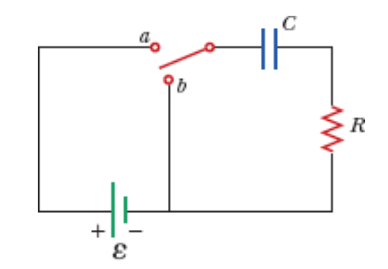
\includegraphics[scale=0.3]{images/theory/circuit.png}
    \end{figure}
    \FloatBarrier
    After the capacitor is charged, we can flip the circuit's switch to position \emph{b} to begin the discharging process, with t=0 now being the time of the circuit closing in position \emph{b}.

    \section{Materials} 
    \begin{enumerate} 
        \item 1 M$\Omega$ resistor
        \item 100$\mu$F polarized capacitor
        \item DC power supply (set at 4V)
        \item Breadboard
        \item Digital multimeter
        \item Dyllan's phone
        \item Numerous alligator clips
        \item Numerous wires 
        \item A single wire that acts as a switch (it's very special)
    \end{enumerate} 


	\section{Experiment Analysis}
    Throughout the experiment, we rely on the following relation between the voltage of the capacitor, the resistance of our resistor, the time constant $\tau$, and time. 
    $$ V_c = \varepsilon (1-e^\frac{-t}{\tau})$$




    \subsection{Linearization of the charging process}
    We start off with our previous equation for the voltage across our capacitor, and begin to manipulate the equation to acquire a more simplified version.

    $$V_c = \varepsilon \left( 1- e^{-\frac{t}{\tau}} \right)  | \div \varepsilon  $$
    $$ \frac{V_c}{\varepsilon}= 1-e^{-\frac{t}{\tau}} $$
    $$ e^{-\frac{t}{\tau}} = 1-\frac{V_c}{\varepsilon} $$
    Take the natural log of both sides.
    $$ -\frac{t}{\tau} = ln\left( 1-\frac{V_c}{\varepsilon}  \right) $$

    We can call the expression $ln(1-\frac{V_C}{\varepsilon})$ our y, and t our x in a linearized equation, to be able to find the time constant, $\tau$, from our plot of voltage and time.  


    



\section{Procedure}
    \subsection{Part 1 - Calculation of the value of the time constant} 
    In this foundational section of the experiment, we measure the functional values of the resistor and the capacitor using the digital multimeter. We then calculated the time constant of our RC circuit using the formula $$\tau = RC$$ and both the theoretical and measure values.
    We finally calculate the percentage error between our theoretical and measure values of the time constant, using the following equation for percentage error. $$\% error = \frac{|\tau_\text{measured} - \tau_\text{nominal}|}{\tau_{nominal}} \times 100$$



    \subsection{Part 2 - Charging the capacitor} 
    After assembling the RC series circuit as displayed in the diagram below and connecting the leads of our multimeter to the leads of the capacitor to get our readouts, we begin the experiment by flipping the switch to the \emph{a} position. When the switch was closed at t=0 seconds, we began recording the voltages across the capacitor at near 5-second intervals. 

    \begin{figure}[hbt!]
        \centering
        \caption{RC series circuit in charging position}
        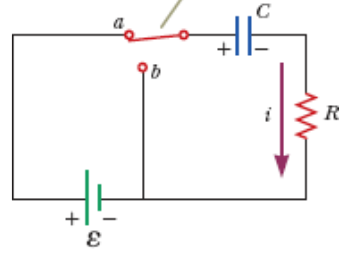
\includegraphics[scale=0.3]{images/procedure/charging.png}
    \end{figure}



    \subsection{Part 3 - discharging the capacitor}
    After performing the previous step of the experiment, we may flip our circuit's switch to the \emph{b} position to begin discharging the capacitor. When the switch is closed at t=0 seconds, we began recording the voltage across the capacitor at roughly 5 second intervals. 
    The following is a link to a recording of the discharging process, with the digital multimeter in view: \url{https://youtu.be/COHm2nRGeQw}.




	\section{Data and Graphs}
	\subsection{Part I: Calculate the value of the time constant}
		The measured value of capacitance of the the capacitor is
		\(\mathbf{ 104.7\pmb{\mu} F }\) \\
		The measured value of the resistor using the DMM is
	\(\pmb{0.987 M\Omega} \)
		\begin{table}[ht!]
			\rowcolors{2}{gray!10}{gray!40}
			\caption*{\textbf{Calculated Time Constants}}
			\centering
			\begin{tabular}{c|c|c}
				$\tau_{measured}$ (sec) & $\tau_{nominal}$ (sec) & \% Error \\
				\hline
				103.34 & 100 & 3.34
			\end{tabular}
		\end{table}

	\subsection{Part II: Charging the capacitor } 
	\begin{minipage}[h]{0.5\textwidth}
		\rowcolors{2}{gray!10}{gray!40}
		\textbf{Voltage v Time for Charging}
		\vspace{1cm}
		\centering
		\begin{tabular}{c|c}
			Time (sec) & Voltage (V) \\
			\hline
			5   & 0.198  \\
			10  & 0.361  \\
			15  & 0.494  \\
			20  & 0.626  \\
			25  & 0.757  \\
			30  & 0.868  \\
			35  & 0.993  \\
			40  & 1.087  \\
			45  & 1.189  \\
			50  & 1.287  \\
			55  & 1.375  \\
			60  & 1.455  \\
			65  & 1.549  \\
			70  & 1.617  \\
			75  & 1.698  \\
			80  & 1.772  \\
			85  & 1.832  \\
			90  & 1.9    \\
			100 & 2.033  \\
			110 & 2.136  \\
			120 & 2.245  \\
			130 & 2.343  \\
			140 & 2.43   \\
			150 & 2.514  \\
			160 & 2.594  \\
			170 & 2.667  \\
			185 & 2.767  \\
			200 & 2.855  \\
			220 & 2.956  \\
			240 & 3.047  \\
			260 & 3.125  \\
			280 & 3.193  \\
			305 & 3.265  \\
			330 & 3.328  \\
			355 & 3.375  \\
			380 & 3.419  \\
			400 & 3.449  \\
			420 & 3.473  \\
			435 & 3.491  \\
			450 & 3.507  \\
			465 & 3.519  \\
			480 & 3.535  \\
			500 & 3.548 \\
			510 & 3.556 \\
			540 & 3.575 \\
			570 & 3.589 \\
			630 & 3.612 \\
			720 & 3.634 \\
			780 & 3.648
		\end{tabular}
		\vspace{14.8cm}
	\end{minipage}
	\begin{minipage}[b]{0.5\textwidth}
		\rowcolors{2}{gray!10}{gray!40}
				\centering
		\textbf{Voltage v Time Linearized}
		\FloatBarrier
				\begin{tabular}{c|c}
					Time (sec) & $-\frac{1}{\tau}$ \\
					\hline
					5   & -0.051  \\
					10  & -0.094  \\
					15  & 0.148   \\
					20  & 0.191   \\
					25  & 0.236   \\
					30  & 0.276   \\
					35  & 0.323   \\
					40  & 0.359   \\
					45  & 0.401   \\
					50  & 0.442   \\
					55  & 0.481   \\
					60  & 0.518   \\
					65  & 0.563   \\
					70  & 0.596   \\
					75  & 0.638   \\
					80  & 0.678   \\
					85  & 0.711   \\
					90  & 0.750   \\
					100 & 0.832   \\
					110 & 0.900   \\
					120 & 0.977   \\
					130 & 1.052   \\
					140 & 1.124   \\
					150 & 1.198   \\
					160 & 1.275   \\
					170 & 1.350   \\
					185 & 1.464   \\
					200 & 1.575   \\
					220 & 1.721   \\
					240 & 1.873   \\
					260 & 2.025   \\
					280 & 2.180   \\
					305 & 2.375   \\
					330 & 2.583   \\
					355 & 2.773   \\
					380 & 2.990   \\
					400 & 3.171   \\
					420 & 3.345   \\
					435 & 3.497   \\
					450 & 3.656   \\
					465 & 3.794   \\
					480 & 4.014  
				\end{tabular}
				\vspace{0.2cm}
			\end{minipage}
			\begin{center}
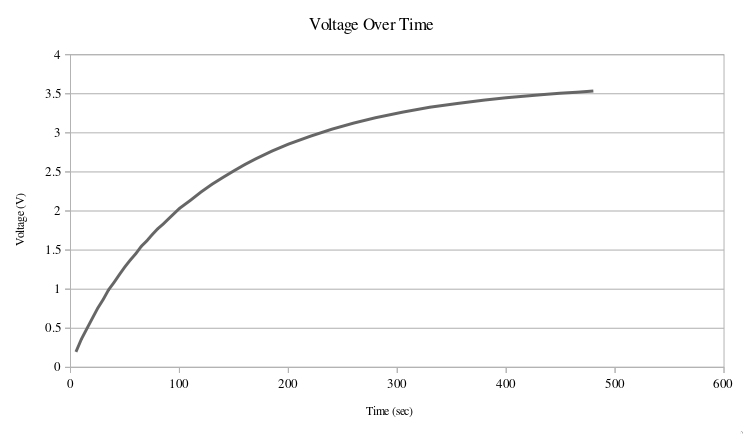
\includegraphics[width=0.9\linewidth,frame]{Voltage-Time.png}
\FloatBarrier
\vspace{1cm}
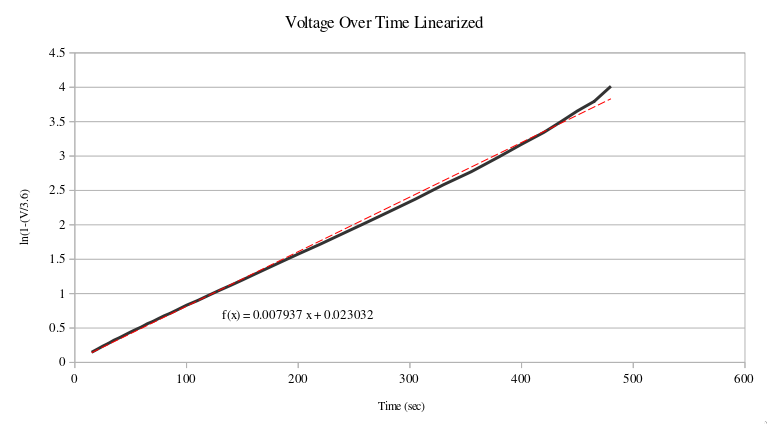
\includegraphics[width=0.9\linewidth,frame]{Voltage-Time-Linear.png}
			\end{center}
			\newpage
	\subsection{Part III: Discharging the capacitor}
			\begin{table}[ht!]
				\rowcolors{2}{gray!10}{gray!40}
				\centering
				\caption*{\textbf{Voltage v Time for Discharging}}
			\begin{tabular}{c|c}
				Time (sec) & Voltage (V)\\
				\hline
				5   & 0.198  \\
				10  & 0.361  \\
				15  & 0.494  \\
				20  & 0.626  \\
				25  & 0.757  \\
				30  & 0.868  \\
				35  & 0.993  \\
				40  & 1.087  \\
				45  & 1.189  \\
				50  & 1.287  \\
				55  & 1.375  \\
				60  & 1.455  \\
				65  & 1.549  \\
				70  & 1.617  \\
				75  & 1.698  \\
				80  & 1.772  \\
				85  & 1.832  \\
				90  & 1.9    \\
				100 & 2.033  \\
				110 & 2.136  \\
				120 & 2.245  \\
				130 & 2.343  \\
				140 & 2.43   \\
				150 & 2.514  \\
				160 & 2.594  \\
				170 & 2.667  \\
				185 & 2.767  \\
				200 & 2.855  \\
				220 & 2.956  \\
				240 & 3.047  \\
				260 & 3.125  \\
				280 & 3.193  \\
				305 & 3.265  \\
				330 & 3.328  \\
				355 & 3.375  \\
				380 & 3.419  \\
				400 & 3.449  \\
				420 & 3.473  \\
				435 & 3.491  \\
				450 & 3.507  \\
				465 & 3.519  \\
				480 & 3.535 
			\end{tabular}
		\end{table}
		\FloatBarrier
		\begin{center}
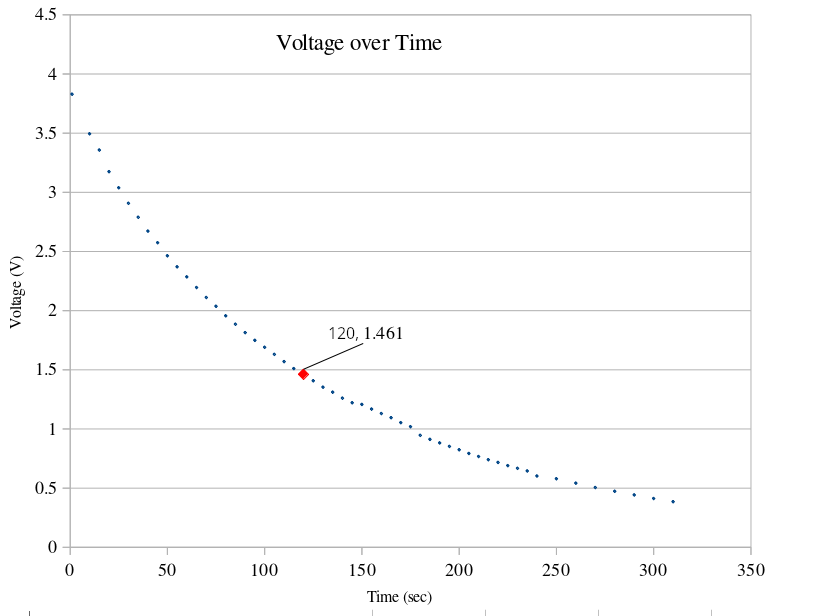
\includegraphics[width=0.9\linewidth,frame]{help.png}
\end{center}
	\subsection{Part IV: Connecting R and C in parallel}
	The voltage read across the resistor with the DMM is \textbf{4.009 V}\\
The voltage read across the capacitor with the DMM is \textbf{4.009 V}\\
	\section{Results}
	\subsection{Part I:Calculate the value of the time constant}
	To calculate the time constant ($\tau$) the resistor is multiplied by the capacitor value via the equation 
	$$\tau = \text{RC}$$
	Substitute the measured values of resistance and capacitance in the equation to recieve the data values stated in Section 5.1.\\
	To calculate the percent error between the expected time constant vs actual time constant created from differing expected resistance and capacitance values, the percent error formula is used
	$$\% error = \frac{|\tau_{measured} - \tau_{nominal}|}{\tau_{nominal}} \times 100$$
	\subsection{Part II: Charging the capacitor}
	In order to linearize the voltage values measured, the following expression is examined:
	$$V_c = \varepsilon \left(1-e^{\frac{-t}{\tau}}\right)$$
	\subsection{Part III: Discharging the capacitor}
	The time constant can be determined by selecting the value of voltage in which it is 37\% of the max voltage (emf). Then, at that point, the time is the time constant. $0.37 \times 4.0$V = $1.48$. The closest point to 1.48 in our graph is 1.461, in which the time is 120 seconds. This means the determined time constant from discharging is 120.
	\subsection{Part IV: Connecting R and C in parallel}
	To calculate the current through the resistor, the equation V = IR is used. Manipulating this equation, current can be found via I = V/R. Using the measured values of resistance and voltage, current can be found as $\frac{4.009V}{0.987M\Omega} = 4.062\mu A$.\\
	The max charge can be calculated using the equation $Q_{max} = C\varepsilon$ substituting values, $104.7\mu F \times 4.009V = 419.7\mu C$
	The energy stored in the capacitor can be found using the equataion $U = \frac{1}{2}C\varepsilon^2$. Substituting values, $\frac{1}{2}104.7\mu F \times 4.009^2 = 841.4\mu J$
	\section{Questions}
    \subsection{Part 4}
    \begin{enumerate}
        \item Do you obtain the same values for the voltage across the resistor and capacitor? Explain.\\ 
            \textbf{Yes! They are in parallel, so the potential difference across each should be the same. If the potential difference wasn’t equal, that wouldn’t make sense, as measuring the potential difference across each one is essentially connecting the multimeter to the same point in the circuit, assuming 0 resistance in the wires.}
        \item Is the current across the resistor zero? Explain.\\ 
            \textbf{No. In the case of the resistor and capacitor being in series, as the capacitor fills up, it blocks the current flow through the resistor. In this configuration, as the capacitor charges more current is simply diverted through the resistor instead of through the capacitor.}



    \end{enumerate}

	\section{Conclusion}
    This lab succeeded in familiarizing our group with the behavior of resistor-capacitor circuits, using both series and parallel configurations.  We were able to plot graphs of the charging and discharging processes, and from those graphs determine the time constant $\tau$. Our group linerized the equation for the charging process, and found the coefficient of that best fit graph. Overall, there were relatively low percentage errors throughout each section of the experiment.




\end{document}
